\section{Alguns elementos do texto}

\subsection[Listas]{Listas {\it \&} Cia.}

itemise, enumerate, description, quotation

\begin{center}\footnotesize\hrule\smallskip
\begin{tabular}{c|c}
\begin{minipage}{.465\textwidth}
\begin{verbatim}
\begin{itemize}
\item cebola,
\item açafrão, e
\item alho.
\end{itemize}
\end{verbatim}
\end{minipage} &
\begin{minipage}{.465\textwidth}
\begin{itemize}
\item cebola,
\item açafrão, e
\item alho.
\end{itemize}
\end{minipage}
\end{tabular}
\smallskip\hrule
\end{center}


\begin{center}\footnotesize\hrule\smallskip
\begin{tabular}{c|c}
\begin{minipage}{.465\textwidth}
\begin{verbatim}
\begin{description}
\item[cebola] Muito empregada p/ temperar.
\item[açafrão] Também.
\item[alho] Idem.
\end{description}
\end{verbatim}
\end{minipage} &
\begin{minipage}{.465\textwidth}
\begin{description}
\item[cebola] Muito empregada p/ temperar.
\item[açafrão] Também.
\item[alho] Idem.
\end{description}
\end{minipage}
\end{tabular}
\smallskip\hrule
\end{center}

\subsection{Alinhamento}\label{sec:alinhamento}

Boa parte dos textos possui alinhamento justificado, i.e., possui
ambas as margens retas e paralelas. Nem sempre isso é
desejado. Existem muitas maneiras de definir o alinhamento do texto:
falamos de duas delas aqui.

\subsection{Texto não-justificado}

\begin{flushleft}
No ambiente
\ambiente{flushleft}\index{flushleft@\ambiente{flushleft}}, o texto é
``empurrado'' para a esquerda. Os espaços não são nem esticados nem
comprimidos. O efeito resultante são linhas de comprimento variável, o
que por vezes é uma opção interessante de diagramação.
\end{flushleft}

\begin{flushright}
Simetricamente,
\ambiente{flushright}\index{flushright@\ambiente{flushright}} tem o
comportamento esperado, fazendo com que o texto no ambiente em
questão, a partir do parágrafo em que aparece, fique com a
esquerda~\emph{rasgada} --- ou seja, para a direita.
\end{flushright}

\subsection{Elementos flutuantes}\label{sec:floats}

Tipógrafos atentam para uma série de características na disposição do
texto que frequentemente passam despercebidas ao nosso consciente. Uma
delas é o equilíbrio entre o texto que se espalha pelas páginas e os
demais elementos, como figuras e tabelas, que pontuam a paisagem aqui
e ali. 

O \LaTeX\ toma várias precauções na disposição desses elementos,
ditos~\emph{flutuantes} (porque sua posição não é fixa no texto como a
de uma palavra em uma frase). É como se os elementos fossem troncos de
árvore à deriva sobre a correnteza de palavras que compõe o texto.

Figuras e tabelas são somente alguns exemplos de elementos
flutuantes. Eles são ambientes (respectivamente~\ambiente{figure}
e~\ambiente{table}) que encapsulam o conteúdo que irá flutuar.

% colocar exemplo usando caption
% enfatizar que o latex sabe onde colocar as imagens
% opções de posicionamento
% todo: como se insere no mecanismo de composição de página

\subsubsection{Figuras}

Figuras são uma ferramenta poderosa na composição de textos, quando
usadas com parcimônia. É possível colocar imagens no documento dizendo
ao \LaTeX\ sua localização (ou apenas seu nome, se estiverem na mesma
pasta que o documento). Também é possível desenhar usando o próprio
\LaTeX, por exemplo, com o pacote \pacote{Tikz}.

Para colocar figuras em um documento \LaTeX, basta usar o comando
\begin{center}
\verb!\includegraphics{nome-do-arquivo}!
\end{center}
em que a extensão do tipo de arquivo não precisa ser incluída. Mas
atenção: nem toda extensão de imagem é conhecida pelo
\LaTeX\ nativamente, embora basta usar um pacote para superar o
problema, na maior parte dos casos. Acrescente
\verb!\usepackage{graphicx}! no preâmbulo de seu documento e você
poderá incluir imagens \extensao{png}, \extensao{jpg} e
\extensao{pdf}, para citar algumas.

\begin{figure}
  \begin{center}
    % From: TeXsample
% The following code is generated by Sketch. I have edited it a bit
% to make it easier to read.
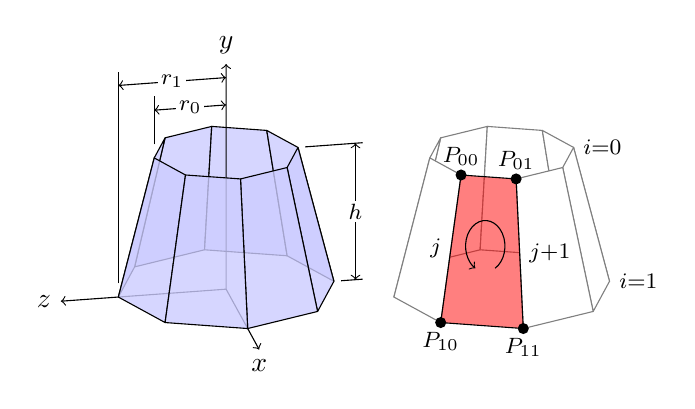
\begin{tikzpicture}[join=round]
    \tikzstyle{conefill} = [fill=blue!20,fill opacity=0.8]
    \tikzstyle{ann} = [fill=white,font=\footnotesize,inner sep=1pt]
    \tikzstyle{ghostfill} = [fill=white]
         \tikzstyle{ghostdraw} = [draw=black!50]
    \filldraw[conefill](-.775,1.922)--(-1.162,.283)--(-.274,.5)
                        --(-.183,2.067)--cycle;
    \filldraw[conefill](-.183,2.067)--(-.274,.5)--(.775,.424)
                        --(.516,2.016)--cycle;
    \filldraw[conefill](.516,2.016)--(.775,.424)--(1.369,.1)
                        --(.913,1.8)--cycle;
    \filldraw[conefill](-.913,1.667)--(-1.369,-.1)--(-1.162,.283)
                        --(-.775,1.922)--cycle;
    \draw(1.461,.107)--(1.734,.127);
    \draw[arrows=<->](1.643,1.853)--(1.643,.12);
    \filldraw[conefill](.913,1.8)--(1.369,.1)--(1.162,-.283)
                        --(.775,1.545)--cycle;
    \draw[arrows=->,line width=.4pt](.274,-.5)--(0,0)--(0,2.86);
    \draw[arrows=-,line width=.4pt](0,0)--(-1.369,-.1);
    \draw[arrows=->,line width=.4pt](-1.369,-.1)--(-2.1,-.153);
    \filldraw[conefill](-.516,1.45)--(-.775,-.424)--(-1.369,-.1)
                        --(-.913,1.667)--cycle;
    \draw(-1.369,.073)--(-1.369,2.76);
    \draw(1.004,1.807)--(1.734,1.86);
    \filldraw[conefill](.775,1.545)--(1.162,-.283)--(.274,-.5)
                        --(.183,1.4)--cycle;
    \draw[arrows=<->](0,2.34)--(-.913,2.273);
    \draw(-.913,1.84)--(-.913,2.447);
    \draw[arrows=<->](0,2.687)--(-1.369,2.587);
    \filldraw[conefill](.183,1.4)--(.274,-.5)--(-.775,-.424)
                        --(-.516,1.45)--cycle;
    \draw[arrows=<-,line width=.4pt](.42,-.767)--(.274,-.5);
    \node[ann] at (-.456,2.307) {$r_0$};
    \node[ann] at (-.685,2.637) {$r_1$};
    \node[ann] at (1.643,.987) {$h$};
    \path (.42,-.767) node[below] {$x$}
        (0,2.86) node[above] {$y$}
        (-2.1,-.153) node[left] {$z$};
    % Second version of the cone
    \begin{scope}[xshift=3.5cm]
    \filldraw[ghostdraw,ghostfill](-.775,1.922)--(-1.162,.283)--(-.274,.5)
                                   --(-.183,2.067)--cycle;
    \filldraw[ghostdraw,ghostfill](-.183,2.067)--(-.274,.5)--(.775,.424) 
                                   --(.516,2.016)--cycle;
    \filldraw[ghostdraw,ghostfill](.516,2.016)--(.775,.424)--(1.369,.1)
                                   --(.913,1.8)--cycle;
    \filldraw[ghostdraw,ghostfill](-.913,1.667)--(-1.369,-.1)--(-1.162,.283)
                                   --(-.775,1.922)--cycle;
    \filldraw[ghostdraw,ghostfill](.913,1.8)--(1.369,.1)--(1.162,-.283)
                                   --(.775,1.545)--cycle;
    \filldraw[ghostdraw,ghostfill](-.516,1.45)--(-.775,-.424)--(-1.369,-.1)
                                   --(-.913,1.667)--cycle;
    \filldraw[ghostdraw,ghostfill](.775,1.545)--(1.162,-.283)--(.274,-.5)
                                   --(.183,1.4)--cycle;
    \filldraw[fill=red,fill
      opacity=0.5](-.516,1.45)--(-.775,-.424)--(.274,-.5)
                                         --(.183,1.4)--cycle;
    \fill(-.775,-.424) circle (2pt);
    \fill(.274,-.5) circle (2pt);
    \fill(-.516,1.45) circle (2pt);
    \fill(.183,1.4) circle (2pt);
    \path[font=\footnotesize]
            (.913,1.8) node[right] {$i\hbox{$=$}0$}
            (1.369,.1) node[right] {$i\hbox{$=$}1$};
    \path[font=\footnotesize]
            (-.645,.513) node[left] {$j$}
            (.228,.45) node[right] {$j\hbox{$+$}1$};
    \draw (-.209,.482)+(-60:.25) [yscale=1.3,->] arc(-60:240:.25);
    \fill[black,font=\footnotesize]
                    (-.516,1.45) node [above] {$P_{00}$}
                    (-.775,-.424) node [below] {$P_{10}$}
                    (.183,1.4) node [above] {$P_{01}$}
                    (.274,-.5) node [below] {$P_{11}$};
    \end{scope}
\end{tikzpicture}

    \caption{Uma figura gerada com o pacote \pacote{Tikz}.}\label{fig:tikz:piramide-cortada}
  \end{center}
\end{figure}


\begin{figure}
  \begin{center}
    \begin{tikzpicture}[scale=.9,every node/.style={minimum size=1cm},on
  grid]
  
    %slanting: production of a set of n 'laminae' to be piled
    %up. N=number of grids.
    \begin{scope}[
            yshift=-83,every node/.append style={
            yslant=0.5,xslant=-1},yslant=0.5,xslant=-1
            ]
        % opacity to prevent graphical interference
        \fill[white,fill opacity=0.9] (0,0) rectangle (5,5);
        \draw[step=4mm, black] (0,0) grid (5,5); %defining grids
        \draw[step=1mm, red!50,thin] (3,1) grid (4,2);  %Nested Grid
        \draw[black,very thick] (0,0) rectangle (5,5);%marking borders
        \fill[red] (0.05,0.05) rectangle (0.35,0.35);
        %Idem as above, for the n-th grid:
    \end{scope}
    
    \begin{scope}[
        yshift=0,every node/.append style={
              yslant=0.5,xslant=-1},yslant=0.5,xslant=-1
                     ]
        \fill[white,fill opacity=.9] (0,0) rectangle (5,5);
        \draw[black,very thick] (0,0) rectangle (5,5);
        \draw[step=5mm, black] (0,0) grid (5,5);
    \end{scope}
    
    \begin{scope}[
        yshift=90,every node/.append style={
          yslant=0.5,xslant=-1},yslant=0.5,xslant=-1
                     ]
      \fill[white,fill opacity=.9] (0,0) rectangle (5,5);
      \draw[step=10mm, black] (1,1) grid (4,4);
      \draw[black,very thick] (1,1) rectangle (4,4);
      \draw[black,dashed] (0,0) rectangle (5,5);
    \end{scope}
    
    \begin{scope}[
        yshift=170,every node/.append style={
              yslant=0.5,xslant=-1},yslant=0.5,xslant=-1
          ]
        \fill[white,fill opacity=0.6] (0,0) rectangle (5,5);
        \draw[step=10mm, black] (2,2) grid (5,5);
        \draw[step=2mm, green] (2,2) grid (3,3);
        \draw[black,very thick] (2,2) rectangle (5,5);
        \draw[black,dashed] (0,0) rectangle (5,5);
    \end{scope}
    
    \begin{scope}[
        yshift=-170,every node/.append style={
        yslant=0.5,xslant=-1},yslant=0.5,xslant=-1
                  ]
        %marking border
        \draw[black,very thick] (0,0) rectangle (5,5);

        %drawing corners (P1,P2, P3): only 3 points needed to define a
        %plane.
        \draw [fill=lime](0,0) circle (.1) ;
        \draw [fill=lime](0,5) circle (.1);
        \draw [fill=lime](5,0) circle (.1);
        \draw [fill=lime](5,5) circle (.1);

        %drawing bathymetric hypotetic countours on the bottom grid:    
        \draw [ultra thick](0,1) parabola bend (2,2) (5,1)  ;
        \draw [dashed] (0,1.5) parabola bend (2.5,2.5) (5,1.5) ;
        \draw [dashed] (0,2) parabola bend (2.7,2.7) (5,2)  ;
        \draw [dashed] (0,2.5) parabola bend (3.5,3.5) (5,2.5)  ;
        \draw [dashed] (0,3.5)  parabola bend (2.75,4.5) (5,3.5);
        \draw [dashed] (0,4)  parabola bend (2.75,4.8) (5,4);
        \draw [dashed] (0,3)  parabola bend (2.75,3.8) (5,3);
        \draw[-latex,thick](2.8,1)node[right]{$\mathsf{Shoreline}$}
                 to[out=180,in=270] (2,1.99);
    \end{scope} %end of drawing grids

    %putting arrows and labels:
    \draw[-latex,thick] (6.2,2) node[right]{$\mathsf{Bathymetry}$}
         to[out=180,in=90] (4,2);

    \draw[-latex,thick](5.8,-.3)node[right]{$\mathsf{Comp.\ G.}$}
        to[out=180,in=90] (3.9,-1);

    \draw[-latex,thick](5.9,5)node[right]{$\mathsf{Wind\ G.}$}
        to[out=180,in=90] (3.6,5);

    \draw[-latex,thick](5.9,8.4)node[right]{$\mathsf{Friction\ G.}$}
        to[out=180,in=90] (3.2,8);

    \draw[-latex,thick,red](5.3,-4.2)node[right]{$\mathsf{G. Cell}$}
        to[out=180,in=90] (0,-2.5);

    \draw[-latex,thick,red](4.3,-1.9)node[right]{$\mathsf{Nested\ G.}$}
        to[out=180,in=90] (2,-.5);

    \draw[-latex,thick](4,-6)node[right]{$\mathsf{Batymetry}$}
    to[out=180,in=90] (2,-5);
    %drawing points on grid's conrners.
    \fill[black,font=\footnotesize]
        (-5,-4.3) node [above] {$P_{1}$}
        (-.3,-5.6) node [below] {$P_{2}$}
    (5.5,-4) node [above] {$P_{3}$};
\end{tikzpicture}

    \caption{Outra figura gerada com o pacote \pacote{Tikz}.}\label{fig:tikz:layers}
  \end{center}
\end{figure}

\subsubsection{Tabelas}\label{sec:tabelas}

\begin{center}
\begin{tabular}{clcr|r|}
  a & b & c & d & e\\
  f & g & h & i & j\\
  \hline
  k & l & m & n & o
\end{tabular}
\end{center}


\begin{table}\centering
  \caption{Gastos {\it \&} despesas / 1º semestre}

  \begin{tabular}{crrrrrrl}
    mês & jan & fev & mar & abr & mai & jun & total\\
    \hline
  receita & $10$ & $0$ & $5$ & $20$ & $12$ & $13$ & $60$\\
  gastos  & $-3$ & $-4$ & $-3$ & $-3$ & $-5$ & $-3$ & $-21$ \\
  \hline
  balanço & $7$ & $-4$ & $2$ & $17$ & $7$ & $10$ & $39$\\
  \end{tabular}
\end{table}
